\documentclass[12pt,a4paper]{report}
%thanks for using LATEX
%Please contact the department to report spelling mistakes or bugs
%Please do not make changes to the main template code without the consent of the HOD, Dept. of EEE
\date{}
\usepackage[hmargin={1.15in,1in},vmargin={1in,1.1in},]{geometry}
%\usepackage[hmargin={1.5in,1.25in},vmargin={1in,1in},]{geometry}
\usepackage{amsmath,graphicx,makeidx,listings,subfigure,float,setspace}
\usepackage{fancyhdr}
\usepackage{sectsty}
\usepackage{lipsum}
\usepackage[final]{pdfpages}
\usepackage{tocloft,pgffor}
\usepackage{titlesec}
\renewcommand{\cftchappresnum}{Chapter }
\AtBeginDocument{\addtolength\cftchapnumwidth{\widthof{\bfseries Chapter}}}
\renewcommand\contentsname{\begin{center}{\large TABLE OF CONTENTS} \end{center} {\normalsize  No. \hfill \normalsize Content  \hfill \normalsize Page}  \vspace{-1cm}}
\renewcommand\listfigurename{\large \begin{center} {LIST OF FIGURES} \end{center} }
\renewcommand\listtablename{\large \begin {center}{LIST OF TABLES} \end{center}}
\setcounter{tocdepth}{1}
%\usepackage{atbegshi}
%\renewcommand\thebibliography{THEBIBLIOGRAPHY}
%---------------------------------FRONT PAGE--------------------------------------------------------------

\pagenumbering{}


\title{{\bf \Large RESPIRATORY RATE ESTIMATION ON EMBEDDED SYSTEM }\\ 
\vspace{0.4cm}
\vspace{1cm}
{\normalsize { SEMINAR REPORT}}\\
{\normalsize{ submitted by }}\\
\vspace{0.3 cm}
{\large\textbf{RIDHIN THOMAS ALEX}}\\
\normalsize {Reg. No:\textbf{ MAC21EE079 }}\\
\vspace{0.25cm}
\normalsize{to}\\ 
\vspace{0.25cm}
\normalsize {the APJ Abdul Kalam Technological University}\\
\normalsize {in partial fulfillment of the requirements for the award of the Degree}\\
\vspace{0.25cm}
\normalsize {of}\\
\vspace{0.25cm}
\normalsize {Bachelor of Technology}\\  
\normalsize {in} \\
\normalsize {\emph{ Electrical and Electronics Engineering} }\\
\vspace{1cm}
\begin{figure}[H]
\centering

\includegraphics[scale=0.7]{Fig 1.png}
\end{figure}
{\large \textbf {Department of Electrical and Electronics Engineering}}\\
\vspace{0.1cm}
\large  \textbf {Mar Athanasius College of Engineering, Kothamangalam}\\
\large  \textbf { Kerala, India 686 666}\\
\vspace{0.25cm}
\author \large \textbf {OCTOBER 2025}}
%-----------------------------------CERTIFICATE-------------------------
\begin{document}
\maketitle
\begin{center}
    {\normalsize\bf{DEPARTMENT OF }}\\
    \vspace{0.1cm} {\normalsize \bf {ELECTRICAL AND ELECTRONICS ENGINEERING}}\\
       \vspace{0.2cm}
{\small \bf {MAR ATHANASIUS COLLEGE OF ENGINEERING, KOTHAMANGALAM}}
\end{center}

\begin{center}
\thispagestyle{empty}

\includegraphics[scale=0.9]{Fig 1.png}\\[7pt]
\large{\bf{CERTIFICATE}}
\end{center}
\onehalfspacing  This is to certify that the report entitled {\textbf{Respiratory Rate Estimation on Embedded System}} submitted by \textbf{Mr.\;Ridhin Thomas Alex} (\textbf{Reg.No.\hspace{0.2cm}MAC22EE079}) to the APJ Abdul Kalam Technological University in partial fulfillment of the requirements for the award of the Degree of Bachelor of Technology in  Electrical and Electronics Engineering is a bonafide record of the seminar carried out by him under our guidance and supervision. This report in any form has not been submitted to any other University or Institute for any purpose.
\vspace{0.8in}
\begin{flushleft}
Prof. Smitha Paulose
%\hfill
%\hspace{1.6cm} Prof. Smitha Paulose
\hfill
Dr. Siny Paul
\end{flushleft}
\begin{flushleft}
Seminar Guide \& Seminar Coordinator
%\hfill 
%\hspace{2.75cm}
%Seminar Coordinator
\hfill
Head of the Department
\end{flushleft}


\vspace{0.99in}
\begin{center}
Dept. Seal
\end{center}
\begin{center}
 03.07.2025   
\end{center}


 %--------------------------------------ACKNOWLEDGMENT------------------------------------------------
\newpage
\pagenumbering{roman}
\setcounter{page}{1}
\begin{verbatim}
\end{verbatim}
\begin{center}
\textbf {\large ACKNOWLEDGEMENT}
\end{center}
\vspace{0.4125in}


\noindent It is a great pleasure to acknowledge all those who have assisted and supported me in successfully completing my seminar. \\ 
\\
\noindent
First of all, I thank God Almighty for his blessings as it is only through his grace that I was able to complete my seminar successfully.\\
\\
\noindent 
I take this opportunity to extend my sincere thanks to my seminar guide Prof. Smitha Paulose, Associate Professor, Department of Electrical and  Electronics Engineering, for her constant support and immense contribution to the success of our seminar.  \\
\\
\noindent
I also extend my sincere thanks to our faculty advisor and seminar coordinator Prof. Smitha Paulose, Associate Professor, Department of Electrical and Electronics Engineering, and all other members of the Department of Electrical and Electronics Engineering for sharing their valuable comments during the preparation of the seminar.\\
\\
\noindent
I am also grateful to Dr.Siny Paul, Head of Electrical and Electronics Engineering Department for the valuable guidance as well as timely advice which helped me a lot during the preparation of the seminar.\\
\\
\noindent I am deeply indebted to Dr.Bos Mathew Jos, Principal, Mar Athanasius College of Engineering, for his encouragement and support.\\
\\
\noindent
I wholeheartedly thank all our classmates for their valuable suggestions and for the spirit of healthy competition that existed between us. 

%-----------------------------------------ABSTRACT--------------------------------------------------------
\newpage
\pagenumbering{roman}
\setcounter{page}{2}
\begin{center}
\textbf {\large ABSTRACT}
\end{center}
\vspace{15pt}
Respiratory Rate Estimation on Embedded System addresses the challenge of implementing real-time respiratory rate (RR) monitoring on resource constrained platforms for wearable healthcare devices. The proposed solution utilizes respiratory induced frequency, intensity, and amplitude variations extracted from the infrared (IR) channel of a photoplethysmography (PPG) sensor, specifically the SEN-15219 board. The system features a signal processing algorithm initially developed in Python and validated using synthetic and publicly available respiration-PPG datasets. A graphical user interface (GUI) was developed to visualize and process sensor data in real time. The algorithm was then ported to an MSP432P401R microcontroller, forming the core of a low-power wearable prototype. RR estimation is performed using a novel Fourier Product (FP) method, yielding a mean absolute error (MAE) of 4.1 rpm using 16-second IR-PPG signal windows. This implementation demonstrates the feasibility of deploying RR monitoring on embedded systems with constrained computational and energy resources, enabling lightweight and autonomous vital sign tracking for mobile health applications.
 
%-----------------------------TABLE OF CONTENTS-----------------------------------------------------------
\newpage
\begin{center}
\title{\bf \large TABLE OF CONTENTS}\\\\
\end{center}
\begin{table}[h]
\begin{tabular}{lllll}
\vspace{0.3cm}
Contents        && \multicolumn{3}{l}{}                                                  Page No.      \\[2pt]                                            
\vspace{0.3cm}
\bf LIST OF TABLES & \multicolumn{3}{l}{}                                              & iv       \\[1pt]
\vspace{0.3cm}
\bf LIST OF FIGURES & \multicolumn{3}{l}{}                                              & v       \\[1pt]
\vspace{0.3cm}
Chapter 1   &\multicolumn{3}{l}{\bf INTRODUCTION}                                  &1        \\[1pt]
\vspace{0.3cm}
Chapter 2      & \multicolumn{3}{l}{\bf LITERATURE REVIEW}                             & 3     \\[1pt]
\vspace{0.3cm}
Chapter 3       & \multicolumn{3}{l}{\bf RR ESTIMATION PIPELINE}                    & 5      \\[1pt]
\vspace{0.3cm}
                & 3.1       & \multicolumn{2}{l}{SIGNAL PREPROCESSING AND FILTERING}                      & 5      \\[1pt]
                \vspace{0.3cm}
                & 3.2       & \multicolumn{2}{l}{PEAK DETECTION AND ANOMALY FILTERING}        & 6      \\[1pt]
                \vspace{0.3cm}
                & 3.3       & \multicolumn{2}{l}{RESAMPLING AND FREQUENCY ANALYSIS}        & 7      \\[1pt]
                \vspace{0.3cm}
               & 3.4       & \multicolumn{2}{l}{FOURIER PRODUCT (FP) ESTIMATOR}        & 7      \\[1pt]
                \vspace{0.3cm}
               
Chapter 4      & \multicolumn{3}{l}{\bf EMBEDDED SYSTEM IMPLEMENTATION}    & 9       \\[1pt]
\vspace{0.2cm}
                & 4.1       & \multicolumn{2}{l}{HARDWARE ARCHITECTURE}                      & 9
                \\[1pt]
                \vspace{0.3cm}
                & 4.2       & \multicolumn{2}{l}{SOFTWARE ARCHITECTURE}   & 11      \\[1pt]
                \vspace{0.3cm}
                & 4.3       & \multicolumn{2}{l}{RESOURCE MANAGEMENT}   & 12      \\[1pt]
                \vspace{0.3cm}
                & 4.4       & \multicolumn{2}{l}{GUI AND REAL-TIME MONITORING INTERFACE}   & 14      \\[1pt]
                \vspace{0.3cm}
                
Chapter 5      & \multicolumn{3}{l}{\bf EXPERIMENTAL RESULTS AND EVALUATION}
                   & 16     \\[1pt]
\vspace{0.3cm}
                & 5.1       & \multicolumn{2}{l}{DATASET AND EVALUATION METRIC }                      & 16
                \\[1pt]
                \vspace{0.3cm}
                & 5.2       & \multicolumn{2}{l}{PERFORMANCE OF RR ESTIMATORS}   & 1      \\[1pt]
                \vspace{0.3cm}
                & 5.3       & \multicolumn{2}{l}{COMPARISON WITH STATE-OF-THE-ART}                      & 17
                \\[1pt]
                \vspace{0.3cm}
               
                
 Chapter 6      & \multicolumn{3}{l}{\bf CONCLUSION}                                    & 18      \\[1pt]
\vspace{0.3cm}               
                
       
\bf REFERENCES      & \multicolumn{3}{l}{}                                              & 19 
\vspace{0.3cm}
\end{tabular}
\end{table}


\newpage
\listoftables
\addcontentsline{toc}{chapter}{LIST OF TABLES}
\addtocontents{lot}{ \hspace{0.4cm} \textbf{No.} \hspace{5cm} 
\textbf{Title} \hfill \textbf{Page }\par}
\newpage
\listoffigures
\addtocontents{lof}{ \hspace{0.4cm} \textbf{No.} \hspace{6cm} \textbf{Title} \hfill \textbf{Page} \par}



   



%----------------------HEADER AND  FOOTER-----------------------------------------------------------------
\newpage
\pagenumbering{arabic}
\setcounter{page}{1}
\pagestyle{fancy}
\lhead{\emph{Respiratory Rate Estimation on Embedded System  }}
\chead{}
\rhead{}
\lfoot{\emph{Department of Electrical and Electronics Engineering, MACE}}
\cfoot{}
\rfoot{\thepage}
\renewcommand{\headrulewidth}{1pt}
\renewcommand{\footrulewidth}{1pt}
\renewcommand{\chaptername}{ \Large {CHAPTER}}
%\renewcommand{\cftchapfont}{16pt}
\chapterfont{\centering}
\renewcommand\bibname{REFERENCES}


%------------INTRODUCTION---------------------------------------------------------------------------------



\chapter{\Large{INTRODUCTION}}


 The paradigm of healthcare is shifting from episodic clinical assessment to continuous, personalized monitoring, a transition driven by the demand for proactive disease management. Within this new framework, the continuous tracking of vital signs outside of traditional hospital settings has become paramount. For individuals managing chronic respiratory conditions, respiratory rate (RR) is a particularly critical metric, as subtle changes in breathing patterns can serve as early indicators of clinical deterioration. Consequently, wearable devices have emerged as an essential technology, offering a convenient and non-invasive means to capture this vital data, thereby enabling timely intervention and reducing the burden of frequent clinical visits.\\

 This technology utilizes a specialized embedded platform that estimates respiratory rate by analyzing photoplethysmography (PPG) signals. These signals reflect blood volume changes influenced by breathing movements \cite{webster1997design}. By applying sophisticated signal processing techniques—particularly spectral analysis methods—the system isolates the breathing-related components within the signals. Extracting features such as frequency shifts and amplitude variations allows accurate determination of respiratory patterns directly from raw sensor data.\\

 A core aspect involves an algorithm that efficiently interprets PPG signals using a Fourier-based approach known as the Fourier Product. This method enhances the identification of dominant respiratory frequencies, offering resilience against noise and artifacts that often affect physiological signals. Implemented on a resource-constrained microcontroller, the algorithm maintains high accuracy while conserving power, making it suitable for portable, low-power wearable devices.\\

 The system employs a PPG sensor module to capture physiological signals, which are then processed by a low-power microcontroller. The embedded software periodically acquires, filters, and analyzes the data before transmitting the results wirelessly to a computer for visualization. The overall setup is designed with an emphasis on portability and energy efficiency, making it well-suited for wearable health monitoring applications. In addition, the design ensures reliable operation under real-time conditions. Such an approach highlights the potential of non-invasive techniques for continuous and convenient monitoring of vital signs. By extracting critical respiratory data from ambient physiological signals with computationally efficient algorithms, the system supports proactive healthcare management, particularly for patients requiring ongoing respiratory surveillance outside clinical settings.\\

  
%---------
%chapter2-------------------------------------------------------------------------------
\chapter{\Large{LITERATURE REVIEW}}

J. Fan et al.\cite{fan2022high} proposed a high-accuracy and ultra-low-power processor for ECG-derived respiration estimation, addressing the common trade-off between accuracy and computational complexity in wearable sensors. Their work introduces several techniques, including QRS detection with refractory period refreshing and adaptive thresholding, to improve performance while minimizing power consumption. Fabricated using a 55 nm process, their processor achieved a record-low power consumption of 354 MW and demonstrated a low estimation error of 0.73 on the CEBS database. The primary contribution of this study is the development of a highly efficient, hardware-based solution for respiration monitoring. However, the research is focused exclusively on ECG signals, meaning its methods are not directly transferable to PPG-based systems without significant adaptation.\\
\\
Bian et al.\cite{bian2020respiratory} presented an end-to-end deep learning approach for estimating RR from PPG signals, utilizing a residual network (ResNet) architecture to automate feature extraction. To address the common issue of limited training data, they augmented their dataset with synthetically generated PPG signals, which improved the model's performance by 34\%. Their final model achieved a mean absolute error of 2.5 rpm on public datasets, a result comparable to classical signal processing methods. The study’s primary contribution is demonstrating that deep learning can effectively learn the complex respiratory modulations in PPG signals without hand-crafted rules. However, the high computational and memory demands of a ResNet architecture make such an approach challenging to deploy in real-time on the low-power, resource-constrained microcontrollers used in wearable devices.\\
\\
Fine et al.\cite{fine2021sources} presented a comprehensive review summarizing the various sources of noise and inaccuracy that affect photoplethysmography (PPG) signals in continuous monitoring applications. Their work categorizes these noise sources into three main groups: individual patient variations (like skin tone, age, and obesity), physiological factors (such as venous pulsation and measurement site), and external perturbations (including motion artifacts, ambient light, and sensor pressure). The primary contribution of this study is to provide a foundational reference for developers, emphasizing that robust wearable devices must account for these realistic noise sources to derive complex clinical parameters accurately. The paper highlights a critical challenge in the field: many systems are tested in controlled environments and fail to address the signal variability encountered in real-world use. \\
\\
Charlton et al.\cite{charlton2016assessment} conducted the first large-scale systematic comparison of algorithms designed to estimate respiratory rate (RR) from both ECG and PPG signals. Their primary aim was to identify the best-performing algorithms under ideal conditions by testing hundreds of different combinations of signal processing techniques. They implemented 314 distinct algorithms—many of which were novel combinations—and evaluated them against a gold-standard reference on data from healthy subjects. Their results showed that the highest-performing algorithms were novel combinations of time-domain estimation and fusion techniques, with several ECG-based algorithms outperforming the clinical standard for continuous monitoring. The study's main contribution is providing a clear benchmark for RR estimation algorithms and releasing a public toolbox to enable reproducible comparisons for future research. A key finding was that, under the tested conditions, algorithms generally achieved higher accuracy when using ECG signals compared to PPG signals.\\
\\
Ravichandran et al.\cite{ravichandran2019respnet} introduced RespNet, a novel end-to-end deep learning model designed to extract the complete respiration signal waveform from PPG, rather than just estimating the respiratory rate. Their network was trained and validated on two separate datasets, demonstrating superior performance over conventional signal processing techniques. The model achieved high cross-correlation coefficients (above 0.93) with reference signals, indicating its ability to accurately reconstruct the respiratory waveform. The primary contribution of this work is its shift in focus from rate estimation to full signal extraction, which could provide richer clinical insights for conditions like sleep apnea. However, as with other deep learning models, RespNet's computational requirements make it unsuitable for direct implementation on the resource-constrained, low-power microcontrollers typical of wearable devices.\\




%------------
%chapter-------------------------------------------------------------------------------
\chapter{\Large{RR ESTIMATION PIPELINE}}

The respiratory rate (RR) estimation pipeline is a structured sequence of signal processing steps designed to extract breathing information from photoplethysmography (PPG) signals. Each stage plays a critical role in refining the raw data, reducing noise, and isolating respiration-related variations. Starting with preprocessing and peak detection, the signal is then resampled to achieve uniform spacing, after which the Fourier Product (FP) estimator identifies the dominant respiratory frequency. Together, these steps enable reliable and efficient estimation of respiratory rate for real-time health monitoring.\\
\section{\large{SIGNAL PREPROCESSING AND FILTERING}}


 Signal preprocessing is the first step in extracting respiratory information from the PPG signal. The raw infrared PPG data is standardized by subtracting the mean and dividing it by its standard deviation. This normalization ensures that variations are independent of baseline shifts or signal magnitude differences.\\

 After standardization, the signal is passed through a band-pass filter (0.1–4 Hz) to retain only the frequency components related to respiration and heart activity while suppressing high-frequency noise and low-frequency drift. For efficiency, two cascaded 4th-order IIR filters are used, making the implementation lightweight and suitable for real-time embedded systems.\\
\begin{figure}[H]
    \centering
    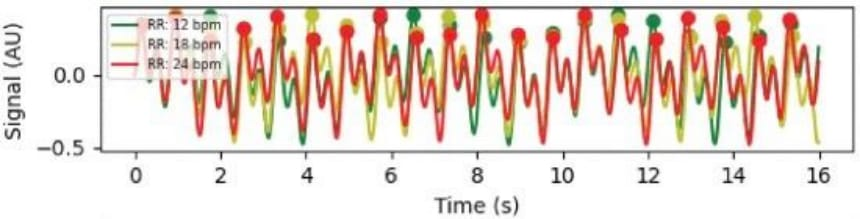
\includegraphics[width=0.7\textwidth]{signal preprocessing.jpg}
    \caption {RR algorithm running in MSP432 processing synthetic PPG signals using RIIV as the estimator. A 16-s window of IR PPG
samples (standardized and filtered).}
    \label{5.10cm}
\end{figure}

 Figure 3.1 shows a 16-second segment of the preprocessed PPG signal. At the top, the raw signal (after standardization and filtering) is plotted, highlighting how noise is reduced and the respiratory-induced variations become clearer. This clean signal forms the input for the next stage, where peaks are detected and analyzed for respiration-related patterns.\\



 \section{\large{PEAK DETECTION AND ANOMALY FILTERING}}

 
 Once the signal is preprocessed, the next step is to identify the peaks that represent significant variations in the PPG waveform. Peaks are detected within non-overlapping 1-second windows using a threshold of 40\% of the maximum peak-to-peak amplitude. This ensures that only physiologically meaningful peaks are considered while ignoring small fluctuations caused by noise.\\

 The detected peaks are stored in a Peak Array (PA) containing their time and intensity values. Since raw detection may include irregular or spurious peaks, an anomaly filter is applied. Peaks that suggest a heart rate lower than 90\% or higher than 115\% of the subject’s actual heart rate are considered abnormal and discarded. The result is a cleaned Peak Intensity Array (PIA), which serves as the input for resampling and frequency analysis.
\begin{figure}[H]
    \centering
    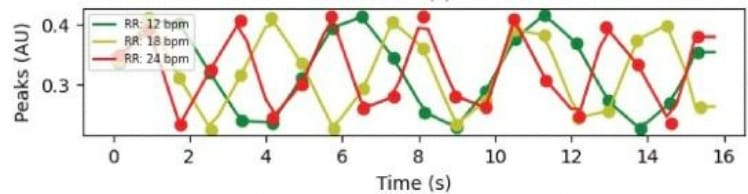
\includegraphics[width=0.7\textwidth]{peak detection.jpg}
    \caption{ Detected peaks at the corresponding signal intensity value and the interpolation.
}
    \label{5.10cm}
\end{figure}
 Figure 3.2 illustrates how peaks are identified and refined. In the top part, the PPG waveform is shown with the detected peaks marked by colored dots at their corresponding intensity values. The interpolation line demonstrates how valid peaks are connected smoothly. This visual clearly shows how the anomaly filter eliminates inconsistent peaks and ensures that only accurate respiration-related variations remain, providing a reliable basis for estimating the respiratory rate. 

\section{\large{RESAMPLING AND FREQUENCY ANALYSIS}}


 After anomaly filtering, the cleaned Peak Intensity Array (PIA) is prepared for frequency-domain analysis. Since the peaks are not evenly spaced in time, they are first resampled to a uniform rate of 4 Hz using linear interpolation. This step converts irregular peak intervals into a smooth, continuous signal suitable for spectral analysis.\\

 Once resampled, the signal undergoes a 512-point Fast Fourier Transform (FFT). The FFT decomposes the signal into its frequency components, and the algorithm searches for the dominant peak within the respiratory frequency range of 8–28 breaths per minute (0.13–0.47 Hz). The corresponding frequency is then converted into respiratory rate by multiplying it by 60, giving the final RR value in breaths per minute.\\
\begin{figure}[H]
    \centering
    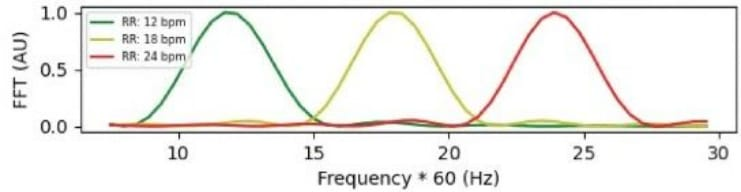
\includegraphics[width=0.7\textwidth]{resampling.jpg}
    \caption{Frequency response of the 4-Hz resampled intensity variability signal. The maximum corresponds to the RR estimation.
}
    \label{5.10cm}
\end{figure}
 Figure 3.3 displays the frequency spectrum of the resampled PIA. On the x-axis is the frequency (converted into respiratory rate range) and the y-axis shows the power or strength of each frequency component. The tallest peak within the 8–28 rpm range represents the subject’s breathing rate. This clear peak demonstrates how the frequency-domain approach highlights the respiratory rhythm while suppressing unrelated variations.
\\
\section{\large{FOURIER PRODUCT (FP) ESTIMATOR}}
 The Fourier Product (FP) estimator is a refinement of the frequency analysis stage that improves accuracy by combining multiple respiration-related variations from the PPG signal. Instead of relying on a single measure, the FP method multiplies the frequency spectra of Respiratory-Induced Intensity Variation (RIIV), Respiratory-Induced Amplitude Variation (RIAV), and Respiratory-Induced Frequency Variation (RIFV) point by point.

    \begin{equation}
S_{\text{FP}}(f) = \mathcal{F}\{\text{RIIV}\} \cdot \mathcal{F}\{\text{RIAV}\} \cdot \mathcal{F}\{\text{RIFV}\}
\end{equation}
    

 This multiplication emphasizes frequency components that are common across all three variations, thereby reinforcing the true respiratory signal while minimizing noise and spurious peaks. Compared to simple averaging, the FP approach is computationally lightweight, does not discard samples, and provides a more robust estimation.

\begin{equation}
\text{RR} = 60 \times \arg\max_{\text{f}} (S_{\text{FP}}(f))
\end{equation}

 In practice, the maximum peak in the product spectrum corresponds to the respiratory frequency, which is then converted into the respiratory rate in breaths per minute. Experimental validation showed that the FP method achieved the lowest Mean Absolute Error ($\approx4.1 rpm$) among all tested approaches, making it both accurate and suitable for real-time embedded systems.\\





%------------
%CHAPTER--------------------------------------------------------------------------------
\chapter{\Large EMBEDDED SYSTEM IMPLEMENTATION}

 The embedded system forms the backbone of the respiratory rate estimation setup, integrating sensors, processing, and communication into a compact and efficient platform. It is designed to operate with low power consumption while maintaining real-time performance, making it suitable for wearable health monitoring applications. The system acquires PPG signals, processes them through an optimized algorithm, and transmits results wirelessly for visualization. Its architecture combines dedicated hardware components with lightweight embedded software, supported by dual-mode operation to balance energy efficiency and responsiveness. In addition, a graphical user interface (GUI) provides real-time monitoring, data storage, and user interaction, completing the end-to-end implementation.\\

\section{\large{HARDWARE ARCHITECTURE}}

The hardware architecture integrates sensing, processing, wireless communication, and power supply into a compact, low-power prototype\cite{martinez2022wearable}. It is optimized for wearable health monitoring, ensuring reliable acquisition of physiological signals, efficient real-time processing, and wireless data transfer, all while maintaining portability and energy efficiency. The assembled prototype, shown in Figure 4.1, visually represents the successful integration of these components into a single, functional unit. The significance of this physical assembly is that it proves the design's feasibility, demonstrating that the individual parts can be combined into a compact and wearable form factor suitable for real-world health monitoring applications.

\begin{figure}[]
    \centering
    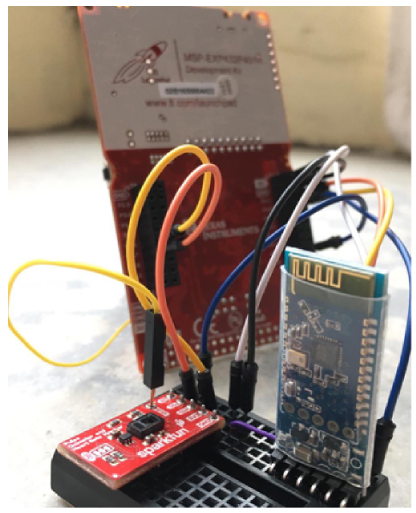
\includegraphics[width=0.3\textwidth]{hardware architech.png}
    \caption{Assembled wearable prototype for real-time RR monitoring}
    \label{5.10cm}
\end{figure}


\subsection{PPG Sensor Module (SEN-15219)}

The system employs the SEN-15219 photoplethysmography sensor board from SparkFun. It uses infrared (IR) and red (R) light emitters along with a photodetector to capture blood volume changes. The module provides continuous measurements of heart rate, oxygen saturation (SpO$_2$), and PPG waveforms, which are further processed to estimate the respiratory rate. The sensor requires a stable power supply and is one of the most energy-demanding parts of the device due to the operation of its LEDs.



\subsection{Microcontroller Unit (MSP432P401R)}

The computational core of the device is the Texas Instruments MSP432P401R, a 32-bit ARM Cortex-M4F MCU running at 48 MHz. It features a hardware floating-point unit for efficient signal processing and supports 93.3 KB of Flash (36.5\%) and 13.5 KB of RAM (17\%) usage for the algorithm. The execution time of the RR estimation algorithm is around 22 ms, enabling real-time performance. The MCU supports dual operation modes—Low Power Mode (LPM0) for energy saving and active mode for high-speed computation.

\subsection{Wireless Communication Module (HC-06 Bluetooth)}

Wireless connectivity is achieved using the HC-06 Bluetooth module, which transmits both raw PPG samples and computed vital signs (RR, HR, SpO$_2$, and temperature) to a PC. Data is sent every 200 ms for waveform visualization and every 1 second for processed values. Bluetooth ensures portability by eliminating wired connections and supports integration with a custom GUI for real-time monitoring.


\subsection{Battery Unit (CR2032 Coin Cell)}

Powered by a 235 mAh CR2032 lithium coin-cell battery, chosen for its compact size and suitability for wearable devices. In continuous mode, the device consumes about 128.8 MWh, giving a runtime of $\sim5.5$ hours. In intermittent mode, where the system wakes every 256 seconds to acquire and transmit data for 32 seconds, the power consumption drops to 38.9 MWh, extending battery life to ~18.2 hours. Among the components, the sensor is the most power-hungry ($\sim43.4\%$ of total consumption), followed by Bluetooth ($\sim33.3\%$) and the MCU ($\sim23.3\%$).




 
\section{\large{SOFTWARE ARCHITECTURE}}


The software architecture is built on a function-queue scheduling mechanism, where tasks are executed at predefined intervals to ensure real-time operation with minimal power consumption\cite{simon1999survey}. After system initialization, the microcontroller enters a low-power mode (LPM0) and wakes only when scheduled events occur. This approach balances computation efficiency with extended battery life, which is essential in wearable devices.
The scheduling is organized as follow:

\begin{itemize}

    \item \textbf{Every 40 ms} → The system acquires and stores new sensor data, updating heart rate and SpO$_2$ values.

    \item \textbf{Every 200 ms} → Infrared PPG samples are added to the RR estimation window and simultaneously transmitted to the Bluetooth module for visualization.

    \item \textbf{Every 1000 ms (1 s)} → Processed values including HR, RR, and SpO$_2$ are sent to the Bluetooth module for external display.

    \item \textbf{Every 16 s }→ The RR estimation algorithm is executed on the collected window, and the RR value is updated.
\end{itemize}

Between these operations, the microcontroller remains in low-power mode, significantly reducing energy consumption. The dual-mode strategy (continuous vs. intermittent operation) further optimizes battery usage, enabling short-term high-resolution monitoring or extended operation depending on user needs.

\begin{figure}[H]
    \centering
    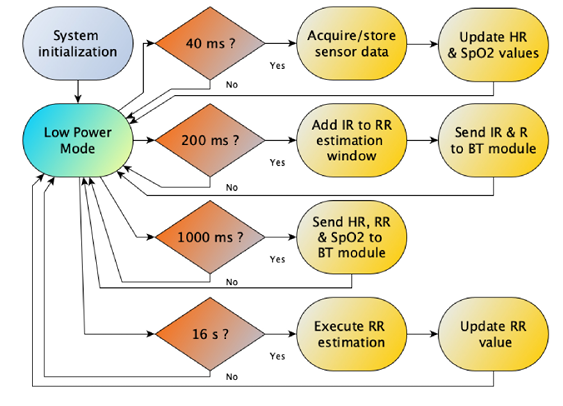
\includegraphics[width=0.6\textwidth]{softaew architecture.png}
    \caption{Embedded software workflow}
    \label{5.10cm}
\end{figure}

Figure 4.2 illustrates the task scheduling flow. After initialization, the system switches to low-power mode and wakes up at defined intervals (40 ms, 200 ms, 1 s, and 16 s) to perform specific operations such as data acquisition, Bluetooth transmission, and RR estimation. This structured timing approach ensures real-time performance while minimizing unnecessary energy use, making the system practical for wearable health monitoring.

\section{\large{RESOURCE MANAGEMENT}}

The successful deployment of any algorithm on a wearable, battery-operated device is critically dependent on efficient resource management. For this prototype, careful consideration was given to the constraints of memory, processing time, and power consumption to ensure its viability for real-world applications. The strategies implemented address the fundamental challenge of balancing computational performance with the need for extended operational autonomy.

\subsection{Memory, Execution Time, and Power Analysis}
A detailed analysis was conducted to quantify the resource demands of the respiratory rate estimation algorithm on the target MSP432P401R microcontroller. This evaluation confirmed the algorithm's suitability for resource-constrained embedded environments.

\begin{itemize}
    \item \textbf{Memory Footprint:} The complete firmware, including the RR estimation algorithm, occupies 93.3 KB of Flash memory, which constitutes 37\% of the total available program space. The run-time memory requirement is 13.5 KB of RAM, or 17\% of the available total. This modest footprint leaves ample resources for future feature enhancements or the integration of additional algorithms without requiring a hardware upgrade.

    \item \textbf{Execution Time:} When operating at its active-mode clock speed of 48 MHz, the microcontroller completes a full 16-second window RR estimation cycle in approximately 22 milliseconds. This rapid execution is crucial for real-time performance. It ensures that the computationally intensive task of RR estimation does not interfere with other time-sensitive operations, such as the periodic 40 ms data sampling from the PPG sensor or the continuous data streaming via the Bluetooth module.

    \item \textbf{Power Analysis:} A breakdown of the system's energy consumption revealed that the most power-hungry component is the SEN-15219 sensor board, primarily due to the power required for its LEDs. In continuous operation, the sensor accounts for 43.4\% of the total energy draw. The HC-06 Bluetooth module is the second-largest consumer at 33.3\%, followed by the MSP432 microcontroller itself, which consumes a relatively modest 23.3\% of the total power. This analysis highlights that further power optimization would most effectively be targeted at the sensor's operational parameters and the data transmission frequency.
\end{itemize}

\subsection{Dual-Mode Operation and Battery Life}
 To provide flexibility for different monitoring scenarios, a dual-mode operational strategy was implemented. This allows the user to choose between high-frequency data collection and extended battery life, making the device adaptable to diverse use cases.

\begin{enumerate}
    \item \textbf{Continuous Mode:} In this mode, the device is always active, continuously acquiring, processing, and transmitting data. This is ideal for applications requiring real-time, high-resolution monitoring, such as in a clinical setting or during physical activity analysis. In this state, the prototype can operate for approximately 5.5 hours on a single CR2032 coin cell battery.
    \item \textbf{Intermittent Mode:} This mode is designed for long-term, ambulatory tracking where continuous data is not necessary. The system wakes from a low-power state (LPM3) to perform a full 32-second data acquisition and transmission cycle once every 256 seconds. This duty-cycled approach dramatically reduces overall power consumption, extending the battery life to approximately 18.2 hours. This makes it suitable for overnight monitoring or tracking daily trends in respiratory rate
\end{enumerate}

Table 4.1 summarizes the key characteristics of each operational mode.
\begin{table}[h!]
\centering
\caption{Dual-Mode Operation of the Prototype}
\label{tab:dual_mode_operation}
\begin{tabular}{|l|l|l|p{5cm}|}
\hline
\textbf{Mode} & \textbf{Sampling Time} & \textbf{Estimated Runtime} & \textbf{Primary Use Case} \\ \hline
Continuous    & Always on              & \textasciitilde{}5.5 hours & Real-time,high-resolution monitoring \\ \hline
Intermittent  & 32s every 256s         & \textasciitilde{}18.2 hours& Long-term,ambulatory tracking      \\ \hline
\end{tabular}
\end{table}

 By implementing these resource management techniques, the prototype demonstrates a practical balance between computational capability and operational longevity, confirming its feasibility as a robust platform for wearable health monitoring.

\section{\large{GUI AND REAL-TIME MONITORING INTERFACE}}

 The Graphical User Interface (GUI) acts as the external monitoring platform for the embedded system. It is designed to receive data packets wirelessly via the Bluetooth module and display both processed physiological values and raw waveforms in real time. The GUI shows heart rate, respiratory rate, oxygen saturation (SpO$_2$), and body temperature as numerical outputs, while simultaneously plotting the PPG waveform for continuous visualization.\\

 Communication is managed using a Python-based application with  the PyBluez library, which handles Bluetooth connectivity and data parsing. Data transfer follows a structured timing sequence: raw PPG samples are transmitted every 200 ms for waveform display, while processed values (HR, RR, SpO$_2$, temperature) are updated every 1 second. This ensures smooth visual updates with minimal delay, allowing both real-time tracking and retrospective analysis of health data.


%------------
%CHAPTER--------------------------------------------------------------------------------
\chapter{\Large EXPERIMENTAL RESULTS AND EVALUATION}

\section{\large{DATASET AND EVALUATION METRIC}}

 The evaluation of the proposed respiratory rate (RR) estimation method was performed using the Beth Israel Deaconess Medical Center (BIDMC) PPG and Respiration dataset, available on the PhysioNet repository\cite{goldberger2000physiobank}. This dataset provides synchronized photoplethysmography (PPG) signals and reference respiration measurements collected from patients in a clinical setting. Since the reference respiration signals serve as reliable ground truth, this dataset is widely used as a benchmark for validating RR estimation algorithms.

 For performance assessment, two key metrics were used:
\begin{itemize}
    \item \textbf{Mean Absolute Error (MAE):} Measures the average deviation between the estimated RR and the reference respiration rate, expressed in respiration per minute (rpm).

    \item \textbf{Standard Deviation (STD):} Quantifies the variability of the estimation error, reflecting the robustness of the method across different subjects and conditions.
\end{itemize}
 By using the BIDMC dataset and these standardized evaluation metrics, the results of the proposed method can be fairly compared with existing state-of-the-art RR estimation algorithms \cite{osathitporn2023rrwavenet}, ensuring objective benchmarking in both accuracy and reliability.


\section{\large{PERFORMANCE OF RR ESTIMATORS}}

 A comparative analysis of several estimation methods was conducted to identify the most accurate and reliable approach for implementation. This investigation revealed clear performance distinctions and underscored the advantages of the proposed fusion technique.
\begin{itemize}
    \item The \textbf{Respiratory-Induced Intensity Variation} (RIIV) estimator, which relies on a single respiratory modulation, was evaluated first as a baseline. It achieved a respectable MAE of 4.38 rpm. While effective, its reliance on a single feature makes it inherently more susceptible to noise that might selectively affect that particular signal characteristic.

    \item An approach using the \textbf{Mean of the RIIV, RIAV, and RIFV} estimators was also tested. This method yielded a slightly higher MAE of 4.42 rpm. Interestingly, it also demonstrated the lowest standard deviation of absolute error, suggesting that while it may not be the most accurate on average, its performance is highly consistent. This consistency comes from the averaging process, which tends to smooth out large, erroneous deviations from any single estimator.

    \item The proposed \textbf{Fourier Product} (FP) method demonstrated superior performance, achieving the lowest MAE of 4.13 rpm. This enhanced accuracy is a direct result of its underlying principle: by multiplying the frequency spectra of the three respiratory modulations, the true respiratory frequency component, which is present and correlated across all three signals, is constructively reinforced. Conversely, noise and artifacts, which are typically random and uncorrelated across the signals, are suppressed. This process effectively acts as a filter, resulting in a cleaner spectrum from which the respiratory rate can be more accurately identified.
    
\end{itemize}

\section{\large{COMPARISON WITH STATE-OF-THE-ART}}

 To contextualize the contribution of this work, the performance of the proposed Fourier Product (FP) method was critically benchmarked against a range of established algorithms, from highly complex deep learning models to other low-complexity signal processing techniques. The results, summarized in Table 5.1, highlight the trade-offs between accuracy, computational complexity, and practical feasibility for wearable devices.

\begin{table*}[h!]
\centering
\caption{Comparison with other RR estimation algorithms.}
\label{tab:stateofart}
\begin{tabular}
{|p{2.75cm}|p{2.5cm}|p{1.45cm}|p{1.75cm}|p{1.85cm}|p{1.15cm}|p{1.15cm}|}

%{|p{2.75cm}|p{2.25cm}|p{2.25cm}|p{2cm}|p{1.75cm}|p{1.25cm}|p{1.25cm}|}
\hline
\textbf{Algorithm} & \textbf{Complexity} & \textbf{RR Range (rpm)} & \textbf{Discard Samples} & \textbf{Window} & \textbf{MAE (rpm)} & \textbf{STD (rpm)} \\ \hline
\textbf{This Work (FP)} & Low & 8--28 & No & 16 s & 4.13 & 3.97 \\ \hline
Karlen et al for this work & Low & 8--28 & Yes & 16 s & 4.51 & 3.78 \\ \hline
Karlen et al in previous work & Low & 4--65 & Yes & 32 s & 5.80 & $>$7.80 \\ \hline
Uguz for this work & Low (AR) & 8--28 & No & 16 s & 4.89 & 4.32 \\ \hline
Pimentel et al & Low (AR) & 4--65 & No & 32 s & 4.00 & $>$3.70 \\ \hline
Bian et al & High & 4--60 & No & 60 s & 2.60 & 0.40 \\ \hline
RRWaveNet & High & ?--65 & No & 16 s & 1.87 & 0.95 \\ \hline
\end{tabular}
\end{table*}

 As shown in the table, high-complexity deep learning models such as RRWaveNet and the method by Bian et al. achieve the highest accuracy, with impressive MAE values of 1.87 rpm and 2.60 rpm, respectively. However, their "High" complexity rating stems from immense computational and memory requirements, making them entirely infeasible for real-time execution on the low-power hardware targeted in this project.\\

 Among the low-complexity algorithms, the proposed FP method demonstrates a superior balance of performance and practicality. When compared to the well-known method by Karlen et al., our implementation yielded a competitive MAE of 4.51 rpm. However, a critical limitation of the Karlen method is its aggressive data rejection strategy. To achieve its accuracy, the algorithm discards signal segments it deems to be of low quality; in our tests, this resulted in the rejection of over 30\% of the data samples. For a continuous monitoring device, such a high rate of data loss is unacceptable. The FP method's ability to achieve a lower MAE of 4.13 rpm without discarding any samples makes it a fundamentally more robust and reliable solution.\\
 
 Furthermore, the algorithm by Pimentel et al. is reported to achieve a slightly lower MAE of 4.00 rpm. This performance, however, comes at the cost of a significant resource requirement: it necessitates a 32-second data window for processing. This doubling of the window size directly translates to a doubling of the RAM required to store the signal buffer, a considerable burden for a low-resource microcontroller where memory is a premium. The FP method's use of a 16-second window makes it far more suitable for memory-constrained systems.\\
 
 The proposed FP method, therefore, successfully carves out a compelling niche. It delivers accuracy that approaches more resource-intensive methods while retaining the computational efficiency, low memory footprint, and complete data integrity essential for a practical and autonomous wearable device.



%------------CONCLUSION-----------------------------------------------------------------------------------
\chapter{ \Large CONCLUSION}

A non-invasive respiratory rate estimation algorithm has been successfully implemented and validated on a low-power embedded system, establishing a highly practical solution for continuous, ambulatory monitoring. The developed prototype effectively bridges the critical gap between computationally intensive deep learning models, which are infeasible for on-device processing, and less robust signal processing techniques that often sacrifice accuracy. By delivering an efficient, end-to-end system centered on a resource-constrained MSP432 microcontroller, this approach demonstrates a balanced and optimized architecture. A key innovation is the introduction of the Fourier Product (FP) estimator, a novel method that enhances estimation accuracy by synergistically combining the frequency spectra of multiple respiratory-induced PPG variations, thereby amplifying the true respiratory signal while suppressing uncorrelated noise. This technique achieves a competitive Mean Absolute Error of 4.13 rpm without the need to discard any data, representing a significant improvement over prior methods that rely on the exclusion of low-quality samples. The resulting power-efficient wearable device, capable of over 18 hours of intermittent operation, ultimately confirms the feasibility of deploying reliable RR estimation for real-world applications in the growing field of wearable health technology, aiding clinicians and users in the long-term management of chronic respiratory conditions and general wellness tracking.

%\tableofcontents
%-----------------REFERENCES------------------------------------------------------------------------------
\bibliographystyle{ieeetr}
\bibliography{references} 
\end{document}